\chapter{Implementierung}

In diesem Kapitel werden die Implementierungen der Funktionstest-Anwendung gemäß der in Kapitel \ref{OOAOOD} erarbeiteten Analyse und Entwurf vorgestellt. Die Anwendung wird insgesamt 4 Mal implementiert: einmal nativ als Referenz und anschließend mit den in Kapitel \ref{Marktanalyse}  vorgestellten 3 Frameworks. Das Hauptaugenmerk liegt hierbei auf den Bereichen, die der Anwendung ein natives Look-And-Feel verleihen sollen. Dies sind entsprechend die Umsetzung der in Kapitel \ref{OOAOODGUI} vorgestellten grafischen Benutzeroberfläche und die Umsetzung der Hardware-Zugriffe für die Nutzung der Sensoren, Kameras und Speicher. So ergeben sich für jede Implementierung 4 Bereiche.

\section{Native Implementierung}

Die native Implementierung der Funktionstest-Anwendung wird mit der IDE 'Android Studio' umgesetzt. Wie schon in Kapitel \ref{AndroidPlattform} beschrieben, ist die Programmiersprache nativer Android Anwendungen Java. Die Anwendung wird gegen die API 23, das bedeutet gegen die Major Version 6 (Marshmallow), kompiliert, da diese Version auch auf dem Testgerät installiert ist. 

\subsection*{Grafische Benutzeroberfläche} \label{natImplGUI}

In Android wird die Struktur der grafischen Benutzeroberfläche über Layouts definiert. Es gibt 2 Wege diese Layouts und ihre Elemente zu deklarieren: Einmal über eine XML-Datei und einmal programmatisch innerhalb der Anwendung über die Nutzung der API. Es wird empfohlen, das Layout über XML-Dateien zu gestalten\footcite{AndroidAPI}, da dies auch eine klarere Trennung der Schicht der grafischen Benutzeroberfläche von der Fachlogikschicht der 3-Schichten-Architektur\footcite{SWTBalzert} begünstigt. 
\\
\\
Für das Hauptmenü und die Auswahl der Sensortests wird, wie in Kapitel \ref{OOAOODGUI} festgelegt wurde, ein 'Navigation Drawer' genutzt. Das Layout dieser Menüs wird in jeweils 3 XML-Dateien beschrieben. Beispielhaft wird an dieser Stelle nur der Code des Hauptmenüs besprochen. Die einzelnen Menüpunkte, die im 'Navigation Drawer' zur Verfügung gestellt werden sollen, werden in der Datei \textit{activity\_main\_drawer.xml} definiert. Wie in unten stehendem Listing \ref{lst:DrawerMenu} dargestellt, wird pro Eintrag im Drawer-Menü ein Item-Objekt definiert. Diesen Item-Objekten werden jeweils eine eindeutige ID, ein Icon und eine Bezeichnung, welche dann im Menü angezeigt wird, übergeben. 

\begin{lstlisting}[caption=Definition der Menüpunkte im 'Navigation Drawer' der Hauptseite in der Datei \textit{activity\_main\_drawer.xml}, label=lst:DrawerMenu, language=XML]
<group android:checkableBehavior="single">      
		...              
        <item
            android:id="@+id/nav_camera"
            android:icon="@drawable/ic_menu_camera"
            android:title="Kamera" />
        <item
            android:id="@+id/nav_gallery"
            android:icon="@drawable/ic_menu_gallery"
            android:title="Gallery" />       
		...               
    </group>
\end{lstlisting} 

Jeder 'Navigation Drawer' hat einen Header. Das Design und der Aufbau dessen wird in der Datei \textit{nav\_header\_main.xml} definiert (siehe Listing \ref{lst:DrawerHeader}). Hier wird bei der Funktionstest-Anwendung der Default-Header von Android Studio genutzt. Für den farbigen Hintergrund, sowie das Android-Icon werden Vorlagen im \textit{drawable}-Ordner mitgeliefert. Diese werden in der Layout-Datei referenziert, wie in Zeile 4 und 11 im unten stehenden Listing \ref{lst:DrawerHeader} zu sehen ist.
\clearpage

\begin{lstlisting}[caption=Definition des Headers des 'Navigation Drawers' in der Datei \textit{nav\_header\_main.xml}, label=lst:DrawerHeader, language=XML]
<LinearLayout xmlns:android="http://schemas.android.com/apk/res/android"
    android:layout_width="match_parent"
    android:layout_height="@dimen/nav_header_height"
    android:background="@drawable/side_nav_bar"    
    ...
    <ImageView
        android:id="@+id/imageView"
        android:layout_width="wrap_content"
        android:layout_height="wrap_content"
        android:paddingTop="@dimen/nav_header_vertical_spacing"
        android:src="@android:drawable/sym_def_app_icon" />

    <TextView
        android:layout_width="match_parent"
        android:layout_height="wrap_content"
        android:paddingTop="@dimen/nav_header_vertical_spacing"
        android:text="Android Studio"
        android:textAppearance="@style/TextAppearance.AppCompat.Body1" />
    ...
</LinearLayout>
\end{lstlisting} 

Das Layout und der Inhalt des 'Navigation Drawers' werden nun in der Layout-Datei des Hauptmenüs, der \textit{MainActivity} referenziert (siehe Listing \ref{lst:MainMenu} Zeile 13 und 14). Hier wird noch über \textit{include} die \textit{App Bar}, die am oberen Bildrand positioniert ist, importiert (siehe Listing \ref{lst:MainMenu} Zeile 2 bis 5). Das \textit{App Bar} Design, welches in der Datei \textit{app\_bar\_main.xml} definiert ist, bringt noch einen \textit{FloatingActionButton} mit sich, der unten rechts im Bildschirm positioniert wird. 

\begin{lstlisting}[caption=Layout des Hauptmenüs in der Datei \textit{activity\_main.xml}, label=lst:MainMenu, language=XML]
...
<include
        layout="@layout/app_bar_main"
        android:layout_width="match_parent"
        android:layout_height="match_parent" />

    <android.support.design.widget.NavigationView
        android:id="@+id/nav_view"
        android:layout_width="wrap_content"
        android:layout_height="match_parent"
        android:layout_gravity="start"
        android:fitsSystemWindows="true"
        app:headerLayout="@layout/nav_header_main"
        app:menu="@menu/activity_main_drawer" />
...
\end{lstlisting} 

Für die Kamerafunktion musste keine eigene Benutzeroberfläche gestaltet werden, da über die API die in Android integrierte Kameraanwendung direkt angesprochen und gestartet wird. Diese Anwendung stellt entsprechend der Anforderungen aus Kapitel \ref{Anforderungsanalyse} sämtliche Benutzereingabemöglichkeiten bezüglich Kamerawechsel oder Blitzeinstellungen zur Verfügung. 
\\
\\
Für die Darstellung der Werte des Beschleunigungssensors wurden \textit{LinearLayout}-Objekte in 3 Ebenen verwendet, welche mit \textit{TextView}-Objekten gefüllt sind, über die die Werte dem Benutzer präsentiert werden. Zur allgemeinen Aufteilung der Layout-Elementen lässt sich sagen, dass die globalen Elemente einer Seite, wie die \textit{AppBar} oder der \textit{FloatingActionButton} in der hierarchisch obersten Layout-Datei \textit{activity\_[name].xml} definiert werden.

\subsection*{Sensoren}

Da die Zugriffe auf die Sensoren und das Auslesen ihrer Daten äquivalent sind werden diese Vorgänge hier am Beispiel des Näherungssensors erläutert. Damit Die \textit{Activity} auf Sensordaten zugreifen kann, braucht sie ein \textit{SensorManager}-Objekt und ein \textit{Sensor}-Objekt (siehe Listing \ref{lst:SensorInit}).

\begin{lstlisting}[caption=Definition und Initialisierung von Sensor und SensorManager, label=lst:SensorInit, language=Java]
private SensorManager mSensorManager;
private Sensor mSensor;
...
mSensorManager = (SensorManager) getSystemService(SENSOR_SERVICE);
mSensor = mSensorManager.getDefaultSensor(Sensor.TYPE_PROXIMITY);
\end{lstlisting} 

Beide Objekte werden direkt beim initialen Start der \textit{Activity} erzeugt. Der \textit{SensorManager} wird benötigt um die \textit{Listener}, welche auf den Sensor horchen, zu registrieren und abzumelden. Dies geschieht in den Methoden \textit{onResume()} und \textit{onPause()} (siehe Listing \ref{lst:onResumeOnPause}). 
\clearpage

\begin{lstlisting}[caption=Die Methoden \textit{onResume()} und \textit{onPause()}, label=lst:onResumeOnPause, language=Java]
protected void onResume() {
        super.onResume();
        mSensorManager.registerListener(this, mSensor,
                SensorManager.SENSOR_DELAY_NORMAL);
}
protected void onPause() {
        super.onPause();
        mSensorManager.unregisterListener(this);
}
\end{lstlisting} 

Die vom Sensor übermittelten Daten werden in einem \textit{SensorEvent}-Objekt der Methode \textit{onSensorChanged()} übergeben. Dort können diese Daten weiterverarbeitet werden. Für die Verarbeitung der Daten des Näherungssensors bedeutet dies, dass dort die Textausgaben 'near' und 'far' generiert werden (siehe Listing \ref{lst:SensorChanged}). 

\begin{lstlisting}[caption=Die Methode \textit{onSensorChanged()}, label=lst:SensorChanged, language=Java]
public void onSensorChanged(SensorEvent event) {
        if (event.values[0] == 0) {
            Toast.makeText(getApplicationContext(), "near", Toast.LENGTH_SHORT).show();
        } else {
            Toast.makeText(getApplicationContext(), "far", Toast.LENGTH_SHORT).show();
        }
}
\end{lstlisting} 

Für den Zugriff auf manche Sensoren und Dienste benötigt die Anwendung eine besondere Erlaubnis. Diese Erlaubnis wird der Anwendung im \textit{AndroidManifest} gegeben. Reicht dies nicht aus, muss eine Anfrage an den Benutzer gestellt werden, welcher dann mit seiner Zustimmung die Erlaubnis erteilt. Im \textit{AndroidManifest} wird diese Erlaubnis über den \textit{uses-permission}-Parameter eingetragen (siehe Listing \ref{lst:usesPermission}).

\begin{lstlisting}[caption=Erlaubnis für die Nutzung eines Dienstes im \textit{AndroidManifest}, label=lst:usesPermission, language=XML]
<uses-permission android:name="android.permission.ACCESS_FINE_LOCATION" />
\end{lstlisting}  

Die Anfrage einer Erlaubnis direkt an den Benutzer wird im Code der jeweiligen \textit{Activity} realisiert, wie in Listing \ref{lst:requestPermission} zu sehen ist:
\clearpage

\begin{lstlisting}[caption=Generierung der Anfrage für die Erlaubnis einen Dienst zu nutzen an den Benutzer, label=lst:requestPermission, language=Java]
...
if (ContextCompat.checkSelfPermission(this, android.Manifest.permission.ACCESS_FINE_LOCATION) != PackageManager.PERMISSION_GRANTED) {
            ActivityCompat.requestPermissions(this,
                    new String[]{android.Manifest.permission.ACCESS_FINE_LOCATION},
                    MY_PERMISSIONS_REQUEST_ACCESS_FINE_LOCATION);
        }
...
\end{lstlisting} 

\subsection*{Kameras}

Wie bereits in Kapitel \ref{natImplGUI} erwähnt, wird für die Kameranutzung die interne Kameraanwendung von Android aufgerufen. Dies geschieht direkt, nachdem vom Hauptmenü aus die Kamerafunktion (\textit{CameraActivity}) aufgerufen wird, also in der \textit{onCreate()}-Methode der \textit{CameraActivity}. Hier ist dieser Aufruf, wie in Listing \ref{lst:callTakeAPic} zu sehen ist in der Methode \textit{takeAPicture()} gekapselt:

\begin{lstlisting}[caption=Aufruf der Android-Kamerafunktion in der \textit{onCreate()}-Methode der Klasse \textit{CameraActivity}, label=lst:callTakeAPic, language=Java]
@Override
    protected void onCreate(Bundle savedInstanceState) {
        super.onCreate(savedInstanceState);
        setContentView(R.layout.activity_camera);

        //dispatchTakePictureIntent();
        _imageView = (ImageView) findViewById(R.id.imageView1);
        takeAPicture();
    }
\end{lstlisting}  

Eine \textit{Activity} wird in Android über einen \textit{Intent} aufgerufen. Ein \textit{Intent} kann auf verschiedene Weisen erzeugt werden. In diesem Fall übergeben wir dem Konstruktor eine \textit{Action} in Form einer \textbf{String}-Variable, nämlich die \textit{ACTION\_IMAGE\_CAPTURE} (siehe Listing \ref{lst:IntentCamera}).
\clearpage

\begin{lstlisting}[caption=Methode \textit{takeAPicture()}: Aufruf der Android-Kamerafunktion über einen \textit{Intent}, label=lst:IntentCamera, language=Java]
private void takeAPicture() {
        Intent intent = new Intent(MediaStore.ACTION_IMAGE_CAPTURE);
        try {
            _file = createImageFile();
        } catch (IOException e) {
            // ToDo
        }
        intent.putExtra(MediaStore.EXTRA_OUTPUT, Uri.fromFile(_file));
        startActivityForResult(intent, REQUEST_IMAGE_CAPTURE);
    }
\end{lstlisting}  

Die Methode \textit{createImageFile()}, welche oben im Listing \ref{lst:IntentCamera} in Zeile 4 aufgerufen wird, generiert Namen für die Bilder, die mit der Kamerafunktion aufgenommen und gespeichert werden. Sollen noch weitere Funktionen ausgeführt werden, sobald ein Bild gespeichert wird, so müssen diese in der Methode \textit{onActivityResult()} definiert werden. Diese Methode wird automatisch immer dann ausgeführt, wenn der Benutzer ein Bild abspeichert. Als Beispiel können hier noch Bildbearbeitungen, wie Formatänderungen, vorgenommen werden, oder das Bild kann, wie Listing \ref{lst:AndroidGallery} zeigt, in der Android \textit{Gallery} zur Verfügung gestellt werden.

\begin{lstlisting}[caption=Bereitstellen des gespeicherten Bildes für die Android \textit{Gallery}, label=lst:AndroidGallery, language=Java]
...
Intent mediaScanIntent = new Intent(Intent.ACTION_MEDIA_SCANNER_SCAN_FILE);
Uri contentUri = Uri.fromFile(this._file);
mediaScanIntent.setData(contentUri);
this.sendBroadcast(mediaScanIntent);
...
\end{lstlisting}  

\subsection*{Speicherzugriffe}

Der in Kapitel \ref{PlanungAnwSpeicher} beschriebene 'External Storage' wird über die Methode \textit{getExternalFilesDir()} andressiert. Da wir in diesem Fall dort Bilder speichern wollen, übergeben wir der Methode dies als Information in Form von \textit{Environment.DIRECTORY\_PICTURES}. In diesem Ordner wird nun der Ordner 'Feature\_Test\_App' erzeugt, wie in Listing \ref{lst:SpeicherZugriff} zu sehen ist.
\clearpage

\begin{lstlisting}[caption=Adressieren des 'External Storage' und Anlegen eines Ordners für die Fotos der Funktionstest-Anwendung, label=lst:SpeicherZugriff, language=Java]
public void CreateDirectoryForPictures() {
        File pubPictures = getExternalFilesDir(Environment.DIRECTORY_PICTURES);
        //this._dir = new File(Environment.getExternalStoragePublicDirectory(Environment.DIRECTORY_PICTURES), "FeatureTestApp");
        CameraActivity._dir = new File(pubPictures, "Feature_Test_App");
        if (!CameraActivity._dir.exists())
        {
            CameraActivity._dir.mkdirs();
        }
    }
\end{lstlisting}

\section{Implementierung mit Xamarin}

Für die Entwicklung von Xamarin Anwendungen auf einem Windows PC wird die IDE 'Visual Studio' verwendet. Die verwendete Programmiersprache ist, wie schon in Kapitel \ref{chpXamarin} erwähnt, C\#. Für den optimalen Vergleich zur nativen Anwendung wird auch die Xamarin-Version gegen die API 23, das bedeutet gegen die Major Version 6 (Marshmallow), kompiliert. 

\subsection*{Grafische Benutzeroberfläche}

Wenn man sich dafür entscheidet in Xamarin eine Anwendung für Android mit den bekannten Android-Bedienelementen zu schreiben, anstelle einer Anwendung mit Xamarin.Forms, so ergibt sich die gleiche Dateistruktur im Projekt wie auch bei der nativen Anwendung. Die Layout-Dateien enden allerdings hier nicht auf .xml, sondern auf .axml. Der interne Aufbau der Layout-Dateien ist identisch mit dem der nativen Layout-Dateien. Möchte man also eine native Anwendung in Xamarin migrieren, ließe sich das Layout ganz einfach übernehmen. 
\\
\\
Um unnötigen doppelten Code auszusparen, wurde ab dieser Implementierung nur noch mit einem \textit{Navigation Drawer} gearbeitet, anstelle von zwei. Da die Inhalte der Layout-Dateien des \textit{Drawers}, wie oben schon erwähnt, identisch mit der nativen Version sind, wird an dieser Stelle auf Ausschnitte dieser verzichtet. Der Zuordnung der einzelnen Seiten der Anwendung zu den Navigationselementen erfolgt ebenfalls ähnlich der nativen Version über \textit{Intents}. Der Code ist bei der Xamarin-Anwendung zwar in C\# geschrieben, die aufgerufene Klasse \textit{Intent} stammt dabei aus dem Android SDK (siehe Listing \ref{lst:ZuordnungNavigationselemente}). 

\begin{lstlisting}[caption=Zuweisung der einzelnen Seiten der Anwendung zu den Navigationselementen im Navigation Drawer, label=lst:ZuordnungNavigationselemente, language=Java]
void NavigationView_NavigationItemSelected(object sender, NavigationView.NavigationItemSelectedEventArgs e)
        {
            switch (e.MenuItem.ItemId)
            {
                case (Resource.Id.nav_camera):
                    Intent intentCamera = new Intent(this, typeof(CameraActivity));
                    StartActivity(intentCamera);
                    break;
                case (Resource.Id.nav_gallery):
                    Intent intentGallery = new Intent(this, typeof(PictureGalleryActivity));
                    StartActivity(intentGallery);
                    break;
                    
                    ...
            }
        }
\end{lstlisting}


In nachfolgender Abbildung \ref{fig:MenuXamarin} ist der \textit{NavigationDrawer} mit den einzelnen Menüpunkten abgebildet. Wie bei der nativen Anwendung ist der \textit{NavigationDrawer} auch in der Xamarin-Anwendung über Wischen und über den Hamburger-Button oben links in der Appbar aus- und wieder einklappbar.
\clearpage

\begin{figure}[h]
	\centering
	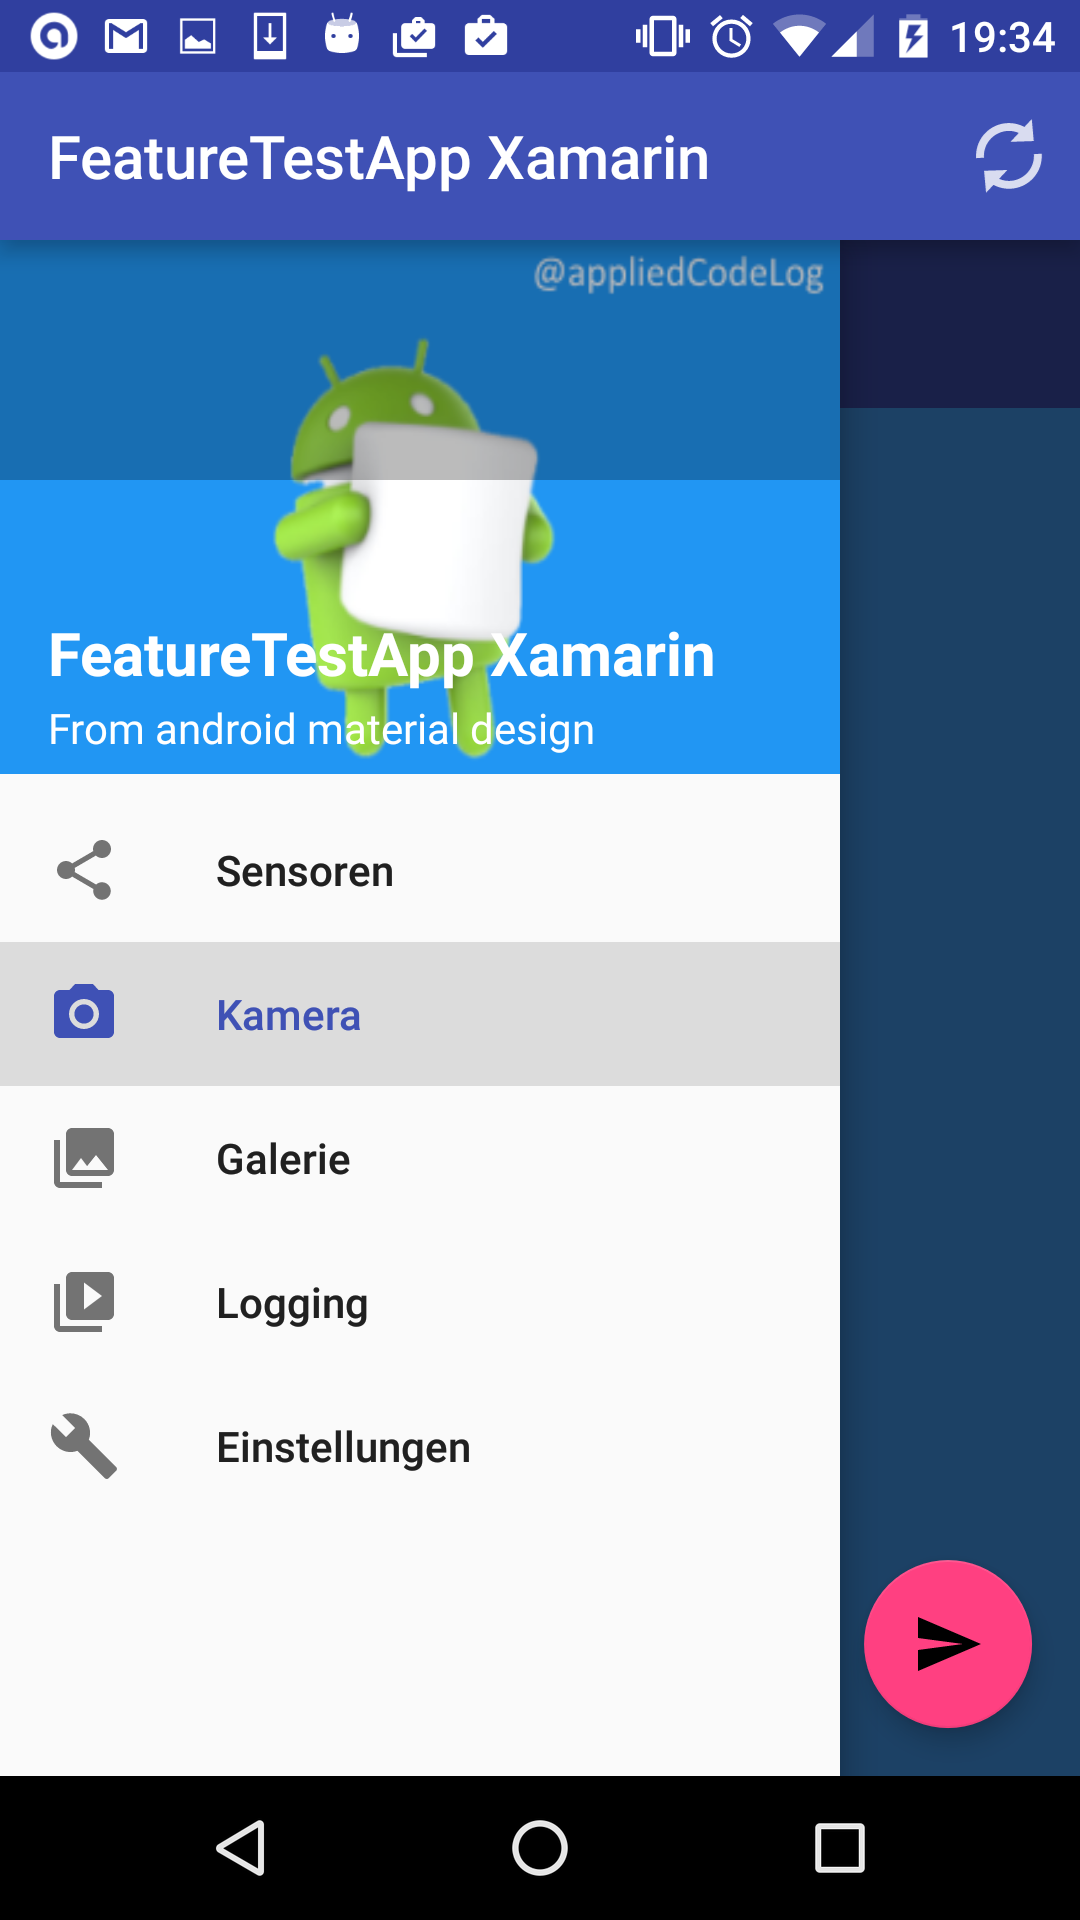
\includegraphics[width=0.4\textwidth]{Bilder/Screenshot_20170328-193448.PNG}
	\caption{Menü in der Xamarin Anwendung}
	\label{fig:MenuXamarin}
\end{figure}

In der Xamarin-Anwendung wird wie in der nativen Anwendung auf der Seite mit der Kamerafunktionalität über die API die in Android integrierte Kameraanwendung direkt angesprochen und gestartet. So verfügt die Anwendung auch über die Möglichkeit des Kamerawechsels und des Einstellen des Blitzes. 
\\
\\
Der \textit{FloatingActionButton} wird wie auch die anderen GUI-Elemente wie der \textit{NavigationDrawer} in einer Layout-Datei deklariert. Da der \textit{FloatingActionButton} auf allen Seiten zur Verfügung stehen soll, wird er wie in der nativen Anwendung in der Layout-Datei \textit{app\_bar.axml} deklariert, welche dann in der Haupt-Layout-Datei importiert wird. Die Deklaration des \textit{FloatingActionButton} ist unten im Listing \ref{lst:FABXamarin} dargestellt. Bei der Deklaration können Farbe, Größe und Positionierung mit angegeben werden. Wie in Kapitel \ref{PlanungAnwGUI} dargestellt, wird in dieser Anwendung der \textit{FloatingActionButton} rechts unten positioniert, was über die Angabe 'bottom|right' geschieht (siehe Listing \ref{lst:FABXamarin}). 
\clearpage

\begin{lstlisting}[caption=Deklaration des \textit{FloatingActionButton} in der Datei \textit{app\_bar.axml}, label=lst:FABXamarin, language=Java]
...
<com.refractored.fab.FloatingActionButton
            android:id="@+id/fab"
            android:layout_width="wrap_content"
            android:layout_height="wrap_content"
            android:layout_gravity="bottom|right"
            android:layout_margin="16dp"
            android:src="@drawable/ic_action_content_new"
            fab:fab_colorNormal="@color/primary"
            fab:fab_colorPressed="@color/primary_pressed"
            fab:fab_colorRipple="@color/ripple" />
...
\end{lstlisting}

\subsection*{Sensoren}

Wie auch bei der nativen Anwendung müssen Berechtigungen im \textit{AndroidManifest} erteilt werden. Hierfür bietet Xamarin in Visual Studio eine grafische Benutzeroberfläche, in der die benötigten Berechtigungen einfach ausgewählt werden können und anschließend automatisch in die Datei \textit{AndroidManifest.xml} eingetragen werden (siehe Abbildung \ref{fig:PermissionsAuswXamarin}). 

\begin{figure}[h]
	\centering
	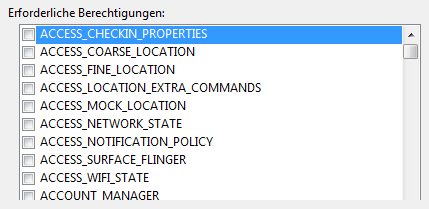
\includegraphics[width=0.7\textwidth]{Bilder/Permissions_Xamarin.PNG}
	\caption{Auswahlfenster für benötigte Berechtigungen in Xamarin (Visual Studio)}
	\label{fig:PermissionsAuswXamarin}
\end{figure}

Der generierte Eintrag in das \textit{AndroidManifest} ist nachfolgend in Listing \ref{lst:usesPermissionXamarin} dargestellt:

\begin{lstlisting}[caption=Erlaubnis für die Nutzung eines Dienstes im \textit{AndroidManifest} (Xamarin), label=lst:usesPermissionXamarin, language=XML]
<uses-permission android:name="android.permission.ACCESS_FINE_LOCATION" />
\end{lstlisting}

Auch das Auslesen von Sensordaten ist nahezu identisch mit der nativen Variante. Für eine gute Vergleichbarkeit bleiben wir auch in diesem Kapitel bei der Vorstellung der Nutzung des Näherungssensors. Wie man in unten stehendem Listing \ref{lst:ProximityXamarin} erkennen kann, ist der Code zum Auslesen der Daten des Näherungssensors praktisch identisch mit dem aus Listing \ref{lst:SensorChanged} (nativ). Auch hier wird die Bearbeitung der Daten in der Methode \textit{onSensorChanged()} der Klasse \textit{SensorEventListener} vorgenommen.

\begin{lstlisting}[caption=Auslesen der Daten des Näherungssensors (Xamarin), label=lst:ProximityXamarin, language=Java]
public void onSensorChanged(SensorEvent event) {
        if (event.values[0] == 0) {
            Toast.MakeText(this, "near", ToastLength.Short).Show();
        } else {
            Toast.MakeText(this, "far", ToastLength.Short).Show();
        }
    }
\end{lstlisting}

\subsection*{Kameras}

Wie bereits oben erwähnt, wird auch bei der Xamarin-Anwendung die im Android SDK integrierte Kameraanwendung aufgerufen und für das Schießen von Fotos verwendet. Ähnlich wie in der nativen Anwendung wurde auch hier eine Methode \textit{TakeAPicture()} geschrieben, in der die Kameraanwendung als \textit{Intent} aufgerufen wird. Dies ist nachfolgend in Listing (X) dargestellt. Wie auch in der nativen Version wird hier über die Klasse \textit{MediaStore} der Standard \textit{Intent ActionImageCapture} aufgerufen, um die Kameraanwendung von Android zu starten. Der Code der Xamarin-Anwendung ähnelt auch an dieser Stelle sehr dem nativen Code, da direkt die Android API für verschiedene Funktionalitäten (in diesem Fall die Kameraanwendung) angesprochen wird.
\clearpage 

\begin{lstlisting}[caption=Methode \textit{TakeAPicture()}: Aufruf der Android-Kamerafunktion über einen \textit{Intent} in Xamarin, label=lst:IntentCameraXamarin, language=Java]
private void TakeAPicture()
        {
            Intent intent = new Intent(MediaStore.ActionImageCapture);
            try
            {
                _file = createImageFile();
            } catch (IOException e)
            ...
        }
\end{lstlisting}

\subsection*{Speicherzugriffe}

Auch bei der Nutzung des \textit{External Storage} ist die Umsetzung mit Xamarin sehr ähnlich der nativen Weise. Auch hier wird die Methode \textit{GetExternalFilesDir} aus der Android API für den Zugriff auf den externen Speicher verwendet. Die Berechtigung für die Nutzung des externen Speichers muss dafür zuvor in das \textit{Android Manifest} eingetragen worden sein (siehe Kapitel (X)). Nachfolgendes Listing (X) zeigt die Implementierung der Methode \textit{GetExternalFilesDir} mit dem Xamarin Framework:

\begin{lstlisting}[caption=Methode \textit{GetExternalFilesDir()}: Adressieren des 'External Storage' und Anlegen eines Ordners für die Fotos der Funktionstest-Anwendung, label=lst:SpeicherzugriffXamarin, language=Java]
private void CreateDirectoryForPictures()
        {
            File pubPictures = GetExternalFilesDir(Environment.DirectoryPictures);
            CameraActivity._dir = new File(pubPictures, "FeatureTestAppXamarin");
            if (!CameraActivity._dir.Exists())
            {
                CameraActivity._dir.Mkdirs();
            }
        }
\end{lstlisting}

\section{Implementierung mit Ionic/Cordova}

Für die Entwicklung mit dem Ionic und Cordova Framework auf einem Windows PC musste zunächst Node.js installiert werden, anschließend wurden sowohl die Ionic und Cordova Kommandozeilen-Tools installiert. Entwickelt wird die Ionic-Anwendung mit JavaScript, hierfür kann ein beliebiger Editor genutzt werden. Auch die Ionic-Anwendung wird für den optimalen Vergleich gegen die API 23, die Major Version 6 (Marshmallow), kompiliert. Hier ist allerdings noch zu erwähnen, dass in der Version Ionic 1 direkt mit JavaScript entwickelt wurde und bei Ionic 2 die von Microsoft entwickelte Programmiersprache TypeScript verwendet wird\footcite{Ionic}, welche auch objektorientierte Prinzipien wie Klassen mit sich bringt. Da jeder JavaScript-Code allerdings auch gültiger TypeScript-Code ist, können weiterhin gängige Javascript-Bibliotheken in TypeScript und somit in Ionic 2 verwendet werden\footcite{TypeScript}. Für diese Arbeit wird Ionic 2 genutzt, da dies die aktuelle Version vom Ionic Framework ist, welche auch weiterentwickelt wird.

\subsection*{Grafische Benutzeroberfläche}

Die Dateistruktur einer Ionic-Anwendung unterscheidet sich sehr stark von einer nativen Android-Anwendung. Dies ist allein schon dadurch bedingt, dass eine Ionic-Anwendung nicht mit einer objektorientierten Programmiersprache, sondern mit der Skriptsprache JavaScript, beziehungsweise TypeScript entwickelt wird.     
\\
\\
Ionic unterstützt verschiedenste UI-Elemente von iOS, Android und Windows, die je nachdem für welche Plattform die Anwendung gebaut wird, automatisch angepasst werden. Das Layout mit seinen einzelnen Elementen wird pro Seite der Anwendung in einer zugehörigen HTML-Datei deklariert. Das Menü mit seinen einzelnen Elementen, in diesem Fall Seiten, wird in der Datei \textit{app.component.ts} deklariert. Diese Datei liegt unter dem Root-Verzeichnis der Anwendung unter src/app/app.component.ts. Hier wird nicht das Design des Menüs festgelegt, sondern nur sein Inhalt mit seinen Bezeichnern. Hierzu müssen die einzelnen Seiten, zu denen man navigieren können soll, importiert werden (siehe Listing (X)). 

\begin{lstlisting}[caption=Import der einzelnen Seiten für die Navigation in der Datei \textit{app.component.ts}, label=lst:app.component.tsImports, language=Java]
import { Page1 } from '../pages/page1/page1';
import { Page2 } from '../pages/page2/page2';
import { Page3 } from '../pages/page3/page3';
import { Page4 } from '../pages/page4/page4';
import { Page5 } from '../pages/page5/page5';
import { Page_main } from '../pages/page_main/page_main';
\end{lstlisting} 

Anschließend werden in dieser Datei noch die Startseite der Anwendung und die Bezeichnungen der Seiten, zu denen man navigieren können soll, gesetzt. Das Benennen der Bezeichnungen und die Zuordnung derer zu den einzelnen Seiten geschieht im Konstruktor (siehe Listing (X)).

\begin{lstlisting}[caption=Setzen der Bezeichnungen der einzelnen Seiten für die Navigation, label=lst:Navigationsbezeichnungen, language=Java]
constructor(public platform: Platform) {
    this.initializeApp();

    this.pages = [
      { title: 'Kamera', component: Page1 },
      { title: 'Galerie', component: Page2 },
      { title: 'Sensoren', component: Page3 },
      { title: 'Logging', component: Page4 },
      { title: 'Manage', component: Page5 }
    ];

  }
\end{lstlisting} 

Das Äquivalent zum \textit{NavigationDrawer} aus Android ist das \textit{Side Menu}. In der Datei \textit{app.html}, welche neben der Datei \textit{app.component.ts} ebenfalls im ordner \textit{src} liegt, wird dieses deklariert. eine Toolbar ist hierbei auch mit integriert. Diese bietet unter anderem den Hamburger-Button, über den sich das \textit{Side Menu} nebst Swipe öffnen lässt. Wird eine Seite ausgewählt, schließt sich das Menü und die neue Seite wird über die in der Datei \textit{app.component.ts} implementierte Methode \textit{openPage()} geöffnet (siehe Listing (X)).

\begin{lstlisting}[caption=Deklaration des \textit{Side Menus} in der Datei \textit{app.html}, label=lst:DeklarationSideMenu, language=html]
<ion-menu [content]="content">
  <ion-header>
    <ion-toolbar>
      <ion-title>Menu</ion-title>
    </ion-toolbar>
  </ion-header>

  <ion-content>
    <ion-list>
      <button menuClose ion-item *ngFor="let p of pages" (click)="openPage(p)">
        {{p.title}}
      </button>
    </ion-list>
  </ion-content>

</ion-menu>
\end{lstlisting}

Nachfolgende Abbildung (X) zeigt das Menü in der Ionic 2 Anwendung. Man kann es wie in der nativen Android Anwendung über Wischen öffnen und schließen. Im Gegensatz zum nativen \textit{NavigationDrawer} und dem von Xamarin, hat das Menü in Ionic nur einen kleinen integrierten Header, der in diesem Fall mit 'Menü' beschriftet ist. 

\begin{figure}[h]
	\centering
	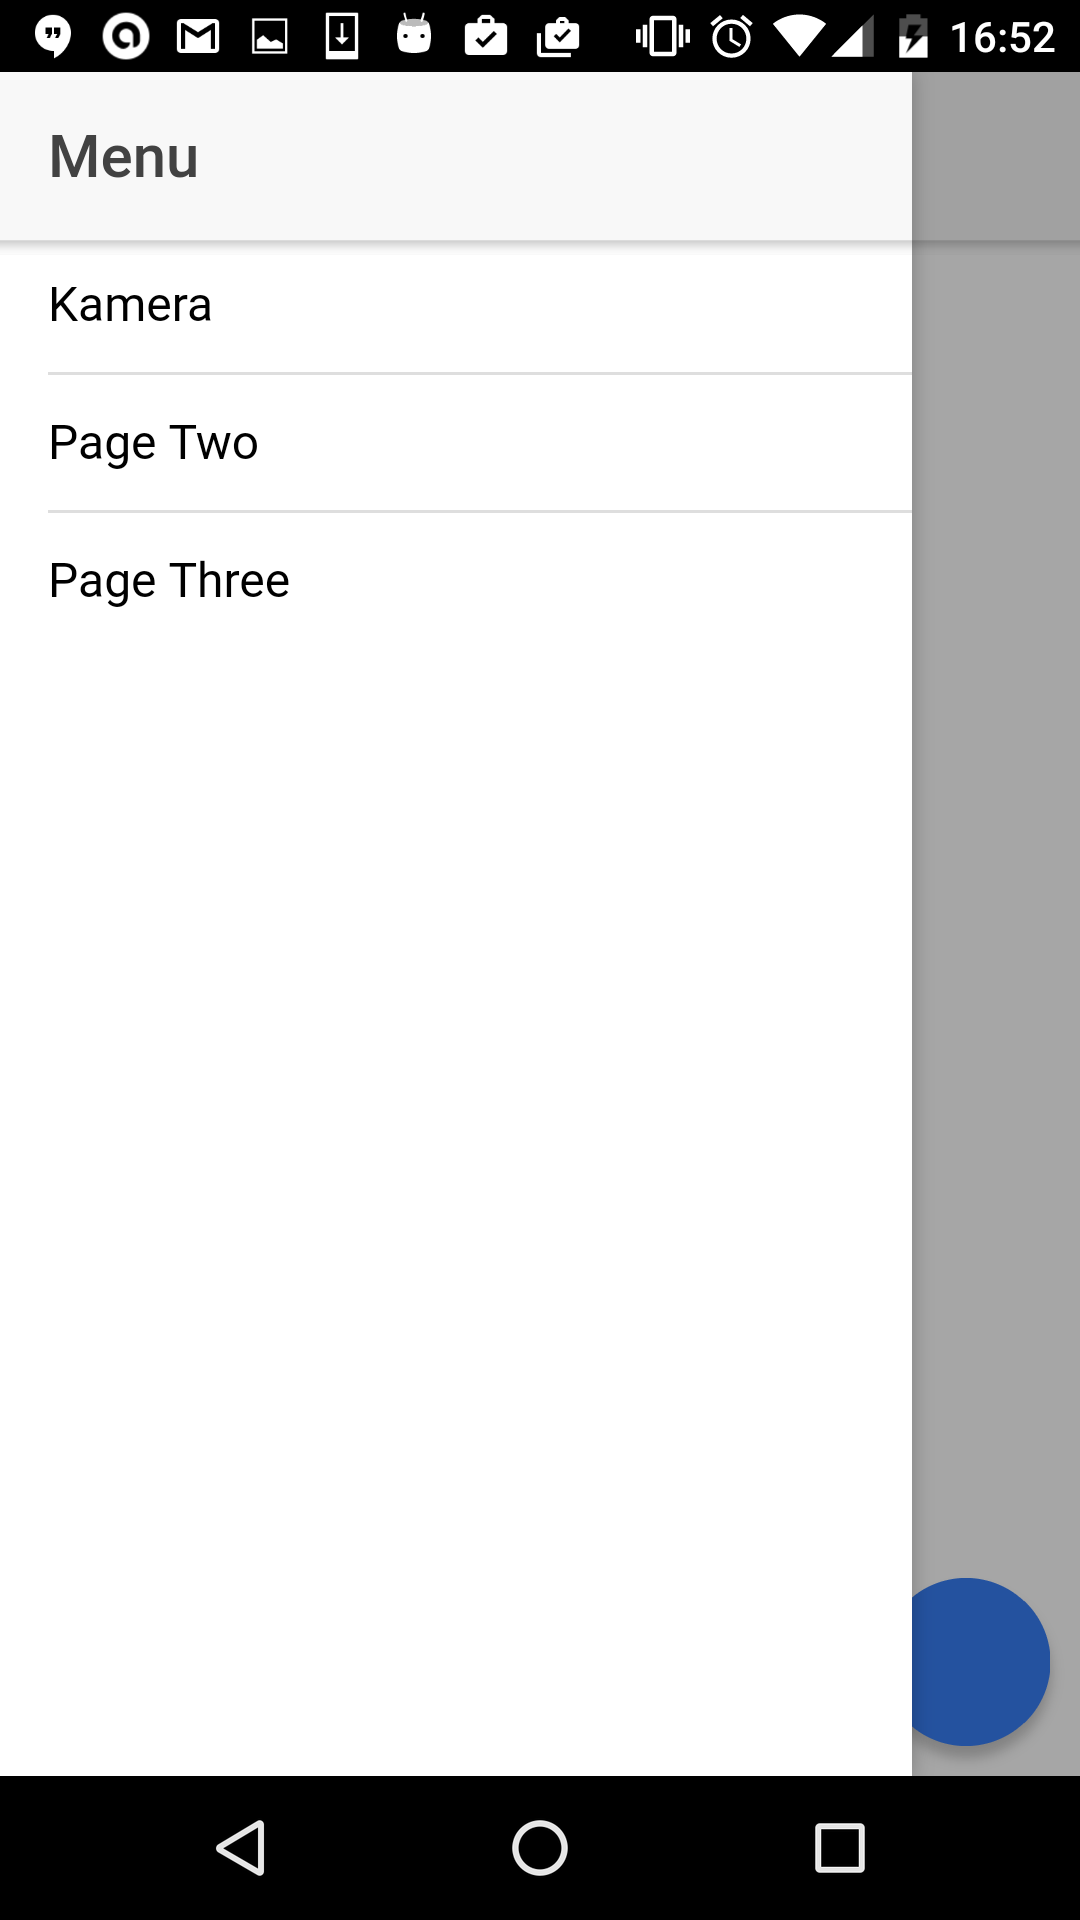
\includegraphics[width=0.4\textwidth]{Bilder/Screenshot_20170328-165235.PNG}
	\caption{Menü in der Ionic 2 Anwendung}
	\label{fig:MenuXamarin}
\end{figure} 

In den HTML-Dateien der einzelnen Seiten, in denen deren Layout definiert wird, muss nur noch seitenspezifisches Design implementiert werden, das Menü wird hier nicht weiter bearbeitet. Das Ionic Framework bietet hier auch direkt die Möglichkeit einen \textit{FloatingActionButton} zu benutzen, was dem nativen GUI-Design entgegenkommt (siehe Listing (X)).

\begin{lstlisting}[caption=Deklaration eines \textit{FloatingActionButton}, label=lst:FloatingActionButtonIonic, language=html]
<ion-fab right bottom>
    <button ion-fab color="red" (click)="presentActionSheet()"></button>
  </ion-fab>
\end{lstlisting}

Im Gegensatz zur nativen Android Entwicklung müssen UI-Elemente, die in der Layout-Datei, hier in einer HTML-Datei, deklariert wurden, nicht mehr im Konstruktor der zugehörigen Source-Datei initialisiert werden. Bei Buttons, die durch Klicken eine Aktion ausführen sollen, wird die auszuführende Methode in der HTML-Datei dem Button zugewiesen, wie oben in Listing (X) zu erkennen ist. 

\subsection*{Sensoren}

Ionic 2 bringt ein \textit{native} Paket mit sich, in dem Klassen definiert sind, welche Cordova-Plugins kapseln und so in TypeScript genutzt werden können. Es existieren bisher nicht für alle Sensoren kapselnde Klassen, sondern nur für den Beschleunigungssensor, das Magnetometer und GPS. Möchte man andere Sensoren nutzen, so ist man darauf angewiesen, ein den Anforderungen entsprechenden Cordova-Plugin zu finden oder ein eben solches selber zu schreiben. Bei der Einbindung und Nutzung eines solchen Cordova-Plugins ist man allerdings wieder dazu gezwungen JavaScript zu nutzen. Dies wird in dieser Arbeit nicht umgesetzt, sondern es wird sich auf das beschränkt, was das Ionic 2 Framework direkt mitliefert.
\\
\\
Um beispielsweise mit Ionic 2 auf das Magnetometer zugreifen zu können, muss zunächst ein bestimmtes Cordova-Plugin installiert werden. Auf der Homepage des Ionic Frameworks sind diese Informationen in der Dokumentation des \textit{native} Pakets zu finden. Im Fall des Magnetometers muss das Plugin \textit{Device Orientation} heruntergeladen und installiert werden. Dies erfolgt über 2 Kommandos (Siehe Listing (X)), welche in einer Kommando-Shell ausgeführt werden müssen, in welcher zunächst in den Root-Ordner der Anwendung navigiert wurde. 

\begin{lstlisting}[caption=Installation des Cordova-Plugins für das Magnetometer, label=lst:InstallationCordovaPlugin, language=bash]
ionic plugin add cordova-plugin-device-orientation
npm install --save @ionic-native/device-orientation
\end{lstlisting}

Anders als bei der nativen Android Entwicklung oder auch bei der Entwicklung mit dem Framework Xamarin, müssen bei der Verwendung von Hardware-Komponenten mit dem Ionic Framework keine Berechtigungen manuell der Anwendung hinzugefügt werden. Die nötigen Berechtigungen bringt das Cordova-Plugin mit sich. Um das installierte Cordova-Plugin in der Anwendung zu nutzen, müssen die dieses Plugin kapselnden Klassen aus dem \textit{native} Paket importiert werden (siehe Listing (X)). 

\begin{lstlisting}[caption=Import der Klassen für die Nutzung des Magnetometers aus dem  \textit{native} Paket von Ionic 2, label=lst:ImportDeviveOrientation, language=Java]
import {DeviceOrientation, DeviceOrientationCompassHeading} from 'ionic-native';
\end{lstlisting}

Anschließend können die importierten Klassen und ihre Methoden dazu genutzt werden, Daten des Sensors auszulesen und anzuzeigen. Um einmalig den aktuellen Wert des Magnetometers auszulesen, kann die Methode \textit{getCurrentHeading()} der Klasse \textit{DeviceOrientation} verwendet werden. Der Rückgabewert dieser Methode ist vom Typ \textit{DeviceOrientationCompassHeading}. Mithilfe der Methode \textit{magneticHeading()} kann nun der aktuelle Sensorwert aus dem \textit{DeviceOrientationCompassHeading}-Objekt gelesen und weiter genutzt werden. Möchte man den Sensor in einem regelmäßigen Intervall auslesen, so wird die Methode \textit{watchHeading()} benötigt. Da es bei einer Kompass-Anwendung sinnvoll ist, immer den aktuellen Sensorwert anzeigen zu lassen ohne manuell aktualisieren zu müssen, werden die Sensordaten hier mittels der Methode \textit{watchHeading()} ausgelesen und angezeigt (siehe Listing(X)). 

\begin{lstlisting}[caption=Auslesen der Daten des Magnetometers mithilfe der Methode \textit{watchHeading()}, label=lst:getDataDeviceOrientation, language=Java]
platform.ready().then(() => {
          DeviceOrientation.watchHeading().subscribe(
            (data: DeviceOrientationCompassHeading) => this.orientation2 = data.magneticHeading.toString()
          );
      });
\end{lstlisting}

\subsection*{Kameras}

Für die Nutzung der Kamera gibt es ähnlich wie oben bei der Sensornutzung beschrieben eine kapselnde Klasse im \textit{native} Paket des Ionic 2 Frameworks. Der Name dieser Klasse ist simpel \textit{Camera}. Um diese Klasse zu nutzen muss ebenfalls wie bei der Sensornutzung vorab ein Cordova-Plugin installiert werden. In diesem Fall ist es das Plugin \textit{Camera}. Die Installation erfolgt über die Kommando-Shell. 
\\
\\
Ruft man die Methode \textit{getPicture()} der Klasse \textit{Camera} auf, so wird über das installierte Cordova-Plugin die native Android Kamera-Anwendung gestartet. Der Methode \textit{getPicture()} können hierbei noch weitere Optionen, zum Beispiel bezüglich der Bildqualität, mitgegeben werden (siehe Listing(X)). 

\begin{lstlisting}[caption=Aufruf der Android Kamera-Anwendung über die Methode \textit{getPicture()}, label=lst:CameraIonic, language=Java]
public takePicture(sourceType) {
  
  var options = {
    quality: 100,
    sourceType: sourceType,
    saveToPhotoAlbum: true,
    correctOrientation: true
  };
	Camera.getPicture(options).then((imagePath) => {
      
        var currentName = imagePath.substr(imagePath.lastIndexOf('/') + 1);
        var correctPath = imagePath.substr(0, imagePath.lastIndexOf('/') + 1);
        this.copyFileToLocalDir(correctPath, currentName, this.createFileName());
      
    }
}
\end{lstlisting}

Wie man oben in Listing (X) sehen kann, wird, nachdem mit der Android Kamera-Anwendung ein Foto geschossen wurde, ein Dateiname mit der Methode \textit{createFileName()} für dieses generiert und die Methode \textit{copyFileToLocalDir} aufgerufen, in der das Speichern dieses Bildes implementiert ist. Die Methode \textit{getPicture()} liefert hier unter anderem den Pfad, unter dem die Android Kamera-Anwendung das Bild zwischenspeichert, zurück.

\subsection*{Speicherzugriffe}

Die Speicherzugriffe zum Speichern und laden geschossener Fotos werden ebenfalls über ein Cordova-Plugin (\textit{File} und \textit{File Transfer}) abgehandelt. Die benötigten Klassen aus dem \textit{native} Paket, welche importiert werden müssen sind \textit{File} und \textit{FilePath}. Wie oben in Listing (X) schon zu sehen war, wird das Speichern in der Methode \textit{copyFileToLocalDir()} vorgenommen. Der Methode werden dafür der aktuelle Pfad, der Name des Bildes und ein neuer Name übergeben. Mit der Methode \textit{copyFile()} wird das Bild nun in dem angegebenen Ordner abgelegt. In diesem Fall ist das \textit{cordova.file.externalDataDirectory}. Das \textit{externalDataDirectory} des Cordova-Plugins entspricht dem \textit{External Storage} von Android. Der eben beschriebene Speichervorgang ist unten in Listing (X) zu sehen. 
\clearpage

\begin{lstlisting}[caption=Methode \textit{copyFileToLocalDir()} zum Speichern der aufgenommenen Bilder, label=lst:SavePictureIonic, language=Java]
private copyFileToLocalDir(namePath, currentName, newFileName) {
    File.copyFile(namePath, currentName, cordova.file.externalDataDirectory, newFileName).then(success => {
      this.lastImage = newFileName;
    }, error => {
      this.presentToast('Error while storing file.');
    });
  }
\end{lstlisting}


\section{Implementierung mit React Native}

Wie schon zuvor bei der Entwicklung mit dem Ionic 2 Framework und Cordova muss auch für die Entwicklung mit dem React Native Framework Node.js installiert sein. Anschließend wird das React Native Kommandozeilen Interface installiert. Eine React Native Anwendung basiert auf React. React, oder auch ReactJS ist ein JavaScript Framework zum Designen von Benutzeroberflächen (Quelle (X)). Der Quellcode ist teilweise in JavaScript, teils in HTML geschrieben. Zum Entwickeln mit React Native kann ein beliebiger Editor verwendet werden. Zum optimalen Vergleich wird auch die React Native Anwendung gegen die API 23, die Major Version 6 (Marshmallow), kompiliert.  

\subsection*{Grafische Benutzeroberfläche}

Im Gegensatz zur Entwicklung mit dem Ionic Framework und auch mit Xamarin, steht die Implementierung der grafischen Benutzeroberfläche und die der Fachlogik nicht in getrennten Dateien. Die grafischen Elemente werden zwar wie bei dem Ionic Framework in HTML implementiert, dieser HTML-Code ist allerdings im JavaScript-Quellcode eingebettet. 
\\
\\
React Native unterstützt bereits einige gängige UI-Elemente, wie zum Beispiel den \textit{FloatingActionButton}. Sollte man allerdings etwas Spezielles benötigen, was nicht in den React Native Bibliotheken enthalten ist, so können auch manuell weitere native Komponenten der Anwendung hinzugefügt werden. Die Basis-Quellcode-Dateien für die beiden Systeme Android und iOS liegen direkt unter dem Root-Verzeichnis der Anwendung. Möchte man ausschließlich gemeinsamen Code verwenden, so kann man eine neue gemeinsame Basis-Quelldatei anlegen und in den plattformspezifischen Dateien diese importieren. 
\\
\\
Für ein wie in Kapitel (X) gefordertes Menü bietet das React Native Framework den sogenannten \textit{DrawerNavigator}. Um diesen zu nutzen muss er zunächst oben in der Basis-Quelldatei importiert werden (siehe Listing (X)).

\begin{lstlisting}[caption=Import der Klasse \textit{DrawerNavigator} für das Menü in React Native, label=lst:ImportDrawerNavigator, language=Java]
import { DrawerNavigator } from 'react-navigation';
\end{lstlisting}

Eine Seite, hier ein Screen, wird durch eine eigene Klasse dargestellt, welche von der Klasse \textit{React.Component} erben muss. Der Titel der Seite wird nebst anderen Einstellungen wie ein Icon in den statischen \textit{navigationOptions} festgelegt (siehe Listing (X)).

\begin{lstlisting}[caption=Festlegen des Seitentitels, label=lst:SeitentitelReactNative, language=Java]
class MyHomeScreen extends React.Component {
  static navigationOptions = {
    drawer: () => ({
      label: 'Home',
      icon: ({ tintColor }) => (
        <Image source={require('./images/ic_home_black_24dp.png')} style={[styles.icon, {tintColor: tintColor}]}/>
      ),
    }),
  }
  ...
}
\end{lstlisting}

Zuletzt müssen die einzelnen Seiten, zu denen man navigieren können soll einem \textit{DrawerNavigator}-Objekt zugeordnet werden. Dies geschieht, wie man in Listing (X) sehen kann in der Konstanten \textit{DrawerApp}. 
\clearpage

\begin{lstlisting}[caption=Konfiguration des \textit{DrawerNavigators}, label=lst:DrawerNavigatorConfig, language=Java]
const DrawerApp = DrawerNavigator({
  Home: {
    screen: MyHomeScreen,
  },
  Kamera: {
    screen: CameraRollGallery,
  },
  Senoren: {
    screen: CameraRollGallery,
  },
  ...
});
\end{lstlisting}

Nachfolgend ist in Abbildung (X) das Menü der React Native Anwendung dargestellt. Es lässt sich wie gewohnt über Wischen öffnen und schließen. Anders als die Menüs der anderen Frameworks und das native Menü hat das Menü der React Native Anwendung keinen integrierten Header.

\begin{figure}[h]
	\centering
	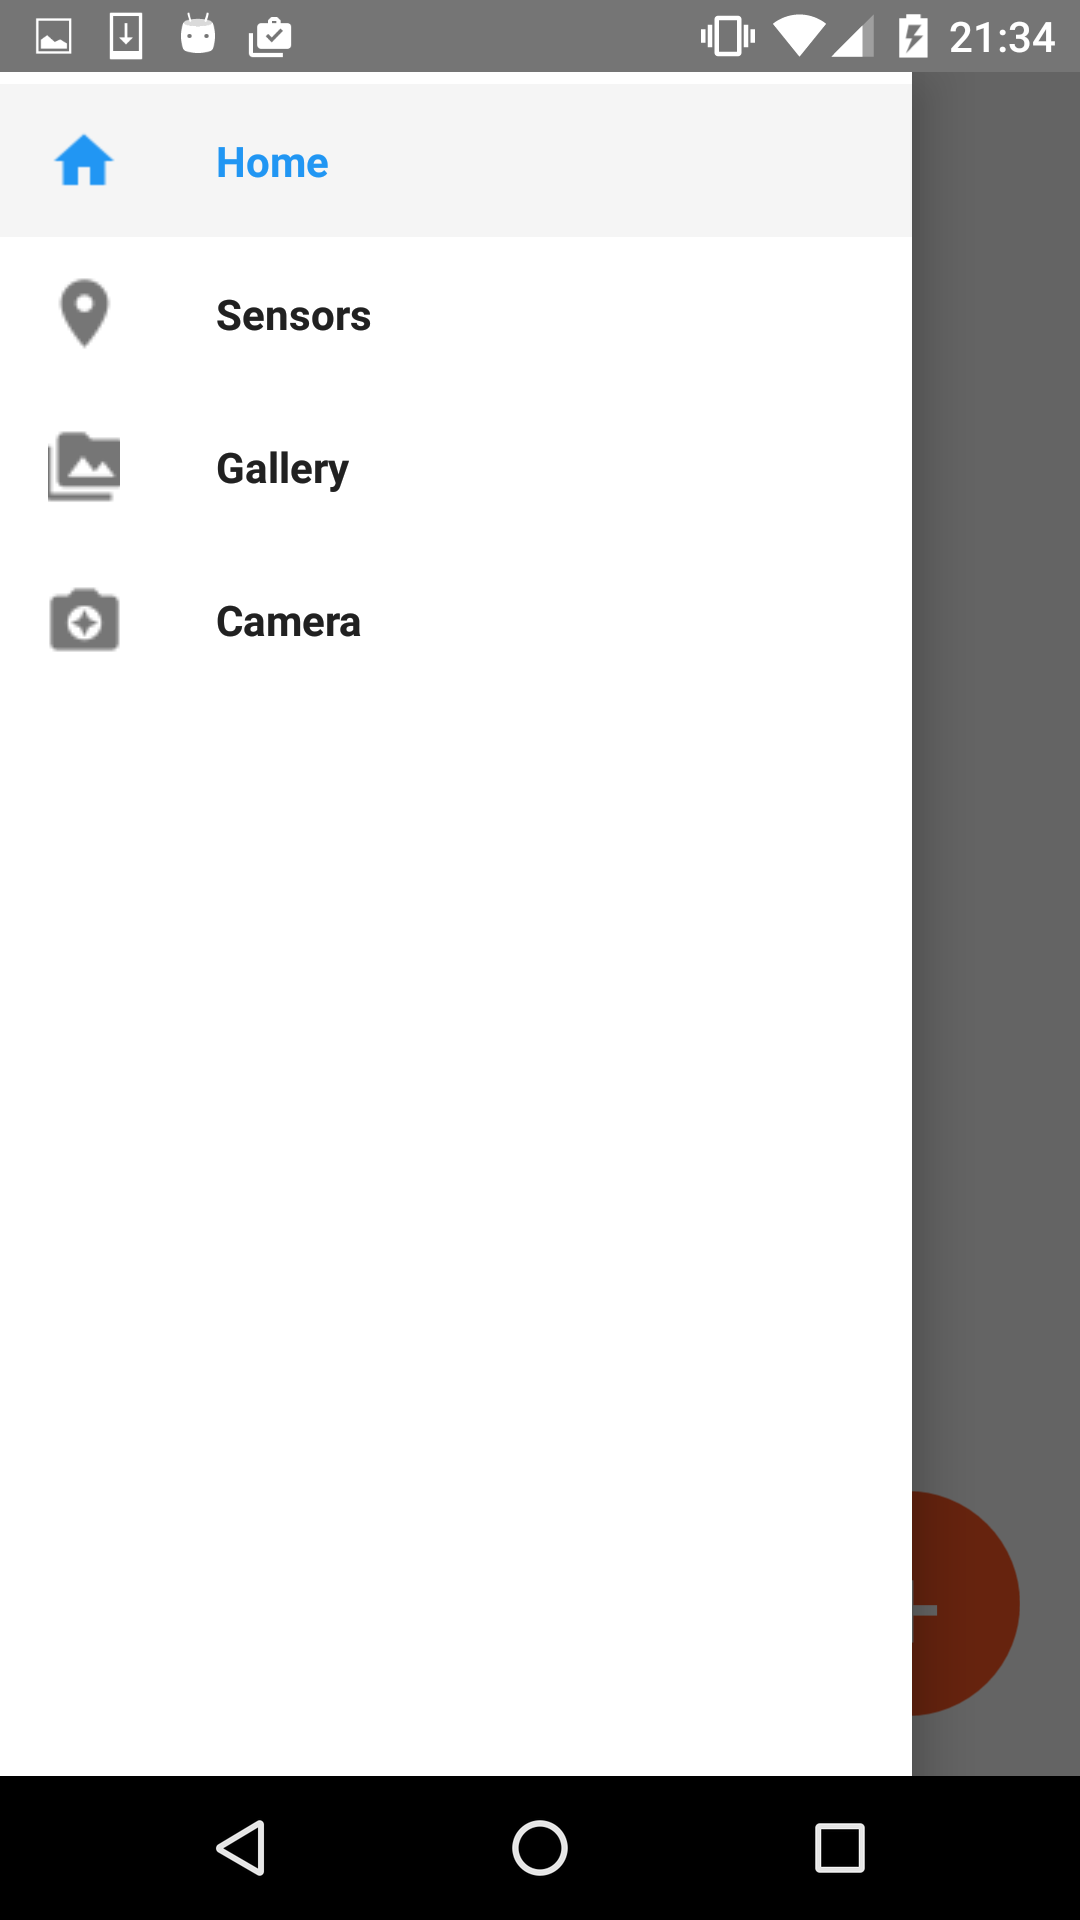
\includegraphics[width=0.4\textwidth]{Bilder/Screenshot_20170412-213445.PNG}
	\caption{Menü in der React Native Anwendung}
	\label{fig:MenuXamarin}
\end{figure}
\clearpage

Einen \textit{FloatingActionButton} bringt das React Native Framework nicht direkt mit. Ein \textit{TouchableHighlight}-Objekt lässt sich allerdings so modifizieren, dass es aussieht und sich verhält wie ein \textit{FloatingActionButton} von Android. Das \textit{TouchableHighlight}-Objekt wird in der \textit{render()}-Funktion der Klasse der Seite deklariert, auf dem der FAB zu sehen sein soll (siehe Listing (X)). 

\begin{lstlisting}[caption=Deklaration eines \textit{TouchableHighlight}-Objekts als \textit{FloatingActionButton}, label=lst:FABReactNative, language=Java]
render() {
    return (
      <TouchableHighlight style={styles.addButton} underlayColor='#ff7043' onPress={() => this.props.navigation.navigate('Camera')}>
        <Text style={{fontSize: 40, color: 'white'}}>+</Text>
      </TouchableHighlight>
    );
  }
\end{lstlisting}

Über \textit{style=styles.addButton} wird dem Objekt sein Design zugeordnet. Das \textit{FloatingActionButton}-Design steckt dabei in dem Attribut \textit{addButton}. In diesem wurden Größe, Form, Position, Verhalten etc. definiert, wie in Listing (X) zu sehen ist.

\begin{lstlisting}[caption=Das \textit{FloatingActionButton}-Design, label=lst:FABDesignReactNative, language=Java]
addButton: {
    backgroundColor: '#ff5722',
    borderColor: '#ff5722',
    borderWidth: 1,
    height: 75,
    width: 75,
    borderRadius: 50,
    alignItems: 'center',
    justifyContent: 'center',
    position: 'absolute',
    bottom: 20,
    right:20,
    shadowColor: "#000000",
    shadowOpacity: 0.8,
    shadowRadius: 2,
    shadowOffset: {
      height: 1,
      width: 0
    }
},
\end{lstlisting} 

\subsection*{Sensoren}

Möchte man in einer React Native Anwendungen auf die Sensoren des Smartphones zugreifen, so bietet sich hierfür die \textit{react-native-sensor-manager}-Bibliothek an. Sensoren, auf die über den Sensor Manager zugegriffen werden können sind: der Beschleunigungssensor, das Gyroskop, das Magnetometer, der Lagesensor, das Thermometer, der Lichtsensor und der Näherungssensor. Das GPS ist direkt über die API des React Native Frameworks ansprechbar. 
\\
\\
Um den Sensor Manager zu nutzen muss dieser zunächst über die Kommando-Shell installiert via \textit{npm} installiert und die Bibliothek verlinkt werden (siehe Listing (X)).

\begin{lstlisting}[caption=Installation und Verlinkung der Bibliothek \textit{react-native-sensor-manager}, label=lst:InstallationSensorManagerRN, language=bash]
npm i react-native-sensor-manager --save
react-native link react-native-sensor-manager
\end{lstlisting}

Fehlen Berechtigungen, so können diese manuell im \textit{AndroidManifest} unter \textit{/android/app/src/main} hinzugefügt werden. Anschließend muss die Klasse \textit{SensorManager} aus dem Paket \textit{NativeModules} in der Quelldatei importiert werden (siehe Listing (X)). 

\begin{lstlisting}[caption=Import der \textit{SensorManager}-Klasse, label=lst:ImportSensorManager, language=Java]
import { SensorManager } from 'NativeModules';
\end{lstlisting}

Das Auslesen und Präsentieren von Sensordaten wird in diesem Fall wieder anhand des Näherungssensors gezeigt. Der Sensor wird im Konstruktor der Seite gestartet, auf der die Daten des Sensors präsentiert werden sollen. Über die Methode \textit{startProximitx()} wird der Näherungssensor gestartet (siehe Listing (X)). Die der Methode übergebene Zahl '100' bedeutet eine Verzögerung von mindestens 100ms zwischen den Events. Mithilfe der Klasse \textit{DeviceEventEmitter} aus der \textit{react-native}-Bibliothek wird ein \textit{Listener} hinzugefügt. 
\clearpage

\begin{lstlisting}[caption=Auslesen und Anzeigen der Daten des Näherungssensors, label=lst:ProximityData, language=Java]
constructor(props) {
    super(props);
    SensorManager.startProximity(100);
    DeviceEventEmitter.addListener('Proximity', function (data) {
        if (data.isNear === true) {
          ToastAndroid.show('Near',ToastAndroid.SHORT);
        } else {
          ToastAndroid.show('Far',ToastAndroid.SHORT);
        }
    });
}
\end{lstlisting}

\subsection*{Kameras}

Um die Kamerafunktionen des Smartphones in einer React Native Anwendung nutzen zu können, muss zunächst die Bibliothek \textit{react-native-camera} via \textit{npm} installiert werden. Anschließend muss die Bibliothek noch mit dem Befehl \textit{react-native link react-native-camera} verknüpft und in der Quelldatei importiert werden. Gegebenenfalls müssen noch Berechtigungen im \textit{AndroidManifest}, welches unter \textit{/android/app/src/main} liegt, hinzugefügt werden. 
\\
\\
Anders als beim Ionic und Xamarin Framework gibt es im React Native Framework direkte Möglichkeit die Android Kameraanwendung innerhalb der React Native Anwendung zu starten. Aus diesem Grund wurden Elemente wie der Auslösebutton und die Blitzeinstellungen manuell der Seite mit der Kamerafunktion hinzugefügt. Die Designs der einzelnen UI-Elemente wurden wie das Design des \textit{FloatingActionButtons} unter \textit{const styles} hinzugefügt. Listing (X) zeigt beispielhaft das Design des Auslösebuttons.

\begin{lstlisting}[caption=Das Design des Auslösebuttons für die Kamerafunktion, label=lst:styleCaptureButton, language=Java]
const styles = StyleSheet.create({
...
captureButton: {
    padding: 15,
    backgroundColor: 'white',
    borderRadius: 40,
  },
...
});
\end{lstlisting} 

In der \textit{render()}-Funktion werden die einzelnen Elemente der Benutzeroberfläche deklariert. Das oben (Listing(X)) gezeigte Design wird hier einem \textit{TouchableOpacity}-Objekt zugeordnet, welches dann den Auslösebutton darstellt (siehe Listing (X)). 

\begin{lstlisting}[caption=Deklaration eines \textit{TouchableOpacity}-UI-Objekts für die Darstellung des Auslösebuttons der Kamera, label=lst:CaptureButton, language=Java]
render() {
    return (
		...
			<TouchableOpacity
                style={styles.captureButton}
                onPress={this.takePicture}
            >
              <Image source={require('./images/ic_photo_camera_36pt.png')}/>
            </TouchableOpacity>
		...
	);
}
\end{lstlisting} 

Wird der Button gedrückt, so wird die Methode \textit{takePicture()} aufgerufen, welche nachfolgend in Listing (X) dargestellt ist. Innerhalb dieser Methode wird die Methode \textit{capture()} des Kameraobjekts \textit{camera} aufgerufen. Dies ist die eigentliche Auslösefunktion der Kamera. Das geschossene Bild wird automatische mit Timestamp im Namen im öffentlichen Bilder-Verzeichnis des Android Smartphones gespeichert. 

\begin{lstlisting}[caption=Die Methode \textit{takePicture()} zum Auslösen der Kamera, label=lst:takePictureReactNative, language=Java]
takePicture = () => {
    if (this.camera) {
      this.camera.capture()
        .then((data) => console.log(data))
        .catch(err => console.error(err));
    }
}
\end{lstlisting} 

Das oben in Listing (X) verwendete Kameraobjekt \textit{camera} wird im Konstruktor der Klasse initialisiert (siehe Listing (X)). Hier werden dem Objekt Voreinstellungen mitgegeben. Beim Start der Kameraanwendung ist in diesem Fall die Rückkamera des Smartphones aktiv und der Blitz ist auf automatisch eingestellt. 
\clearpage

\begin{lstlisting}[caption=Initialisierung des Kameraobjekts im Konstruktor, label=lst:InitialisierungCameraRN, language=Java]
...
camera: {
        aspect: Camera.constants.Aspect.fill,
        captureTarget: Camera.constants.CaptureTarget.cameraRoll,
        type: Camera.constants.Type.back,
        orientation: Camera.constants.Orientation.auto,
        flashMode: Camera.constants.FlashMode.auto,
},
isRecording: false
...
\end{lstlisting}

Für das Ändern des Blitzmodus wird ein UI-Element, welches selbst den aktuell ausgewählten Blitzmodus anzeigt, oben rechts im Bild gesetzt. Durch tippen auf dieses Element wird durch die 3 verschiedenen Blitzoptionen \textit{on}, \textit{off} und \textit{auto} rotiert. Listing (X) zeigt die Initialisierung dieses Elements.  

\begin{lstlisting}[caption=Initialisierung des UI-Elements zum Wechseln des Blitzmodus, label=lst:FlashSwitchElement, language=Java]
...
<TouchableOpacity
	style={styles.flashButton}
    onPress={this.switchFlash}
>
    <Image source={this.flashIcon}/>
</TouchableOpacity>
...
\end{lstlisting}

Die Methode \textit{switchFlash()} übernimmt das Rotieren durch die Blitzoptionen. Wie man in Listing (X) erkennen kann, besitzt das Kameraobjekt ein Attribut \textit{flashMode}, welches entsprechend dem momentan ausgewählten Modus bei Aufruf der Methode \textit{switchFlash()} einen anderen Modus zugewiesen bekommt. Die Methode \textit{flashIcon()} ist wie die Methode \textit{switchFlash()} aufgebaut, nur das in ihr das entsprechende Icon des UI-Elements für die Blitzoptionen gesetzt wird.
\clearpage

\begin{lstlisting}[caption=Die Methode \textit{switchFlash()} für das Ändern des Blitzmodus, label=lst:switchFlash, language=Java]
switchFlash = () => {
    let newFlashMode;
    const { auto, on, off } = Camera.constants.FlashMode;

    if (this.state.camera.flashMode === auto) {
      newFlashMode = on;
    } else if (this.state.camera.flashMode === on) {
      newFlashMode = off;
    } else if (this.state.camera.flashMode === off) {
      newFlashMode = auto;
    }

    this.setState({
      camera: {
        ...this.state.camera,
        flashMode: newFlashMode,
      },
    });
}
\end{lstlisting}

Die manuell erstellte Benutzeroberfläche für die Bedienung der Kamerafunktionen in der React Native Anwendung ist nachfolgend in Abbildung (X) dargestellt. In der linken oberen Ecke ist das Element zum Wechseln zwischen Rück- und Frontkamera. Die Funktionsweise dieses Elements entspricht der der Blitzoptionen. 
\clearpage

\begin{figure}[h]
	\centering
	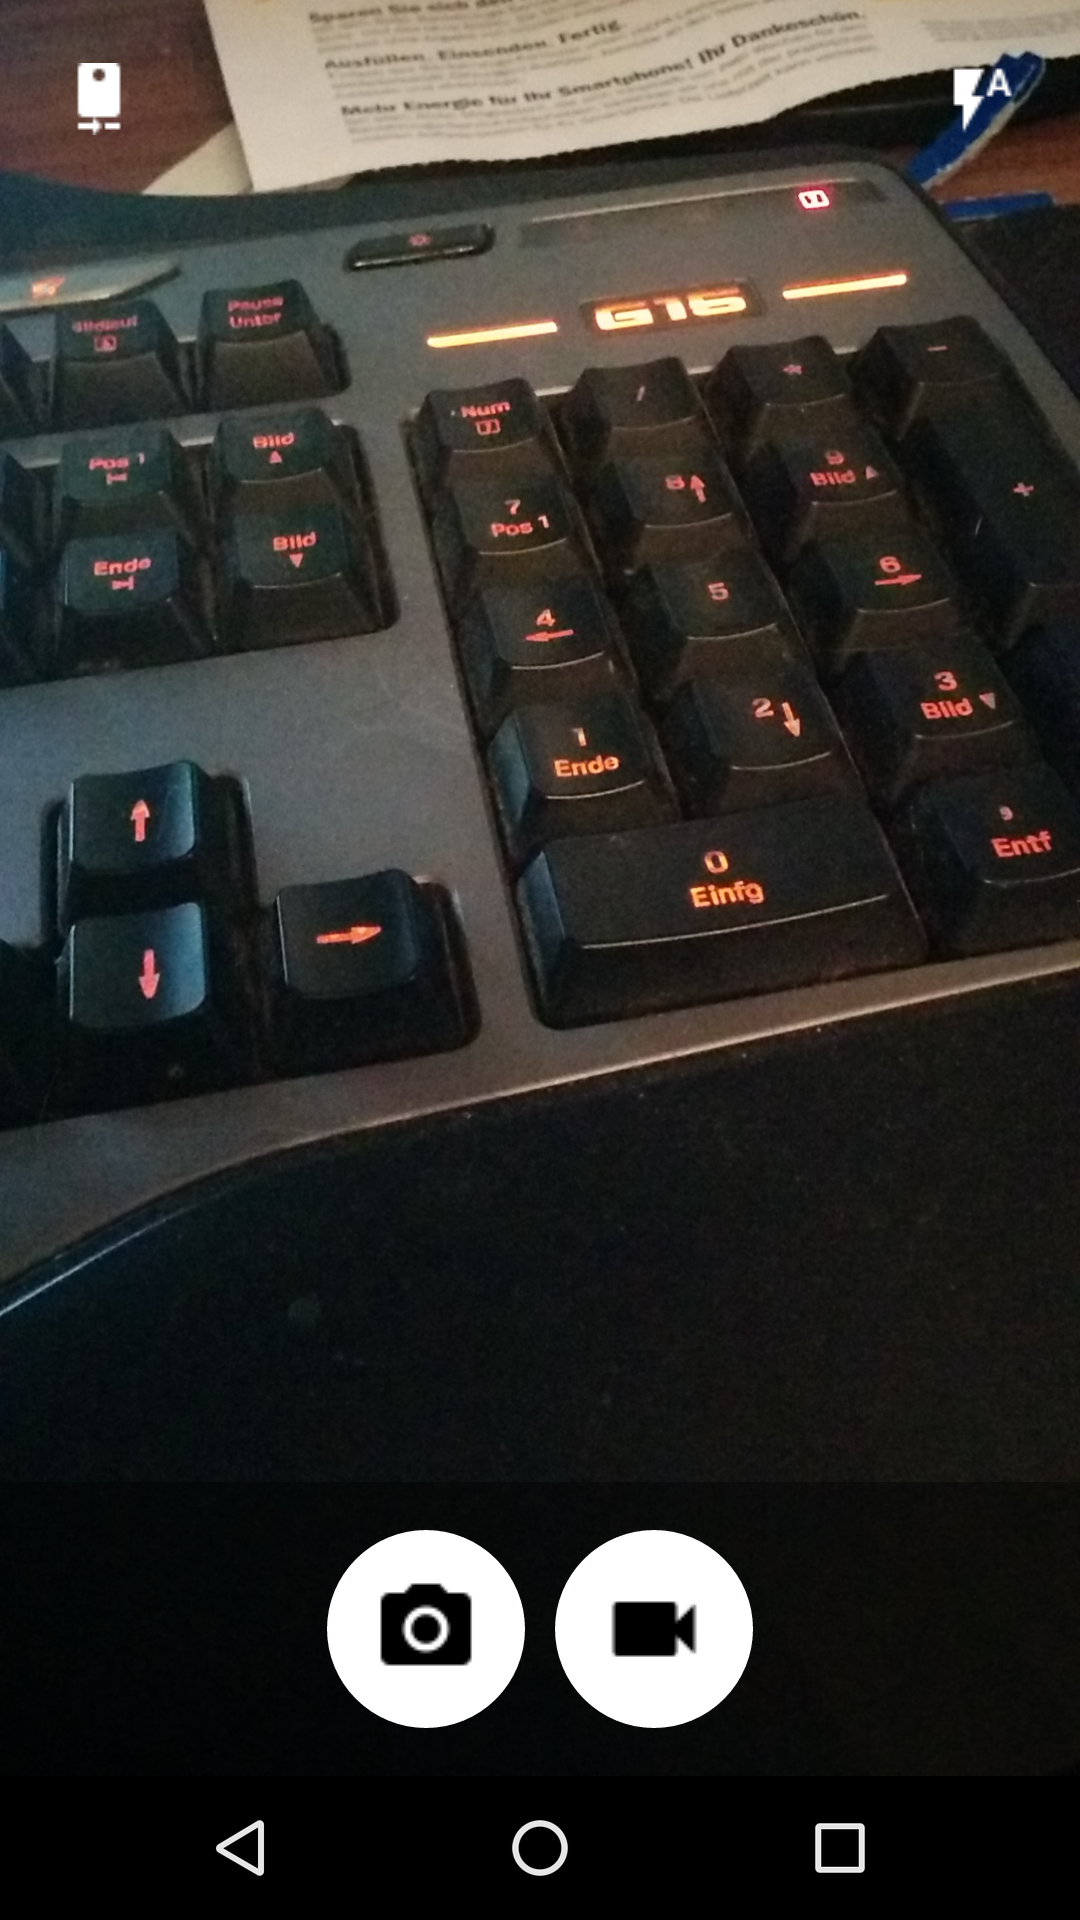
\includegraphics[width=0.4\textwidth]{Bilder/Screenshot_20170412-213200.PNG}
	\caption{Kamerafunktion in der React Native Anwendung}
	\label{fig:KameraReact}
\end{figure}

\subsection*{Speicherzugriffe}

Um die geschossenen Fotos, oder bei Bedarf auch weitere Bilder, die Auf dem Smartphone gespeichert sind, zu laden wird die Methode \textit{getPhotos()} der Klasse \textit{CameraRoll} aufgerufen (siehe Listing (X)). Die Klasse \textit{CameraRoll} ist aus dem Plugin \textit{rn-camera-roll}, welches zuvor über \textit{npm} installiert und anschließend in der Quelldatei importiert werden musste. Der Methode \textit{getPhotos()} können hierbei verschiedene Optionen mitgegeben werden, die unter anderem angeben, welche Bilddateien geladen werden sollen. Ein paar Möglichkeiten sind hier \textit{Library}, \textit{All} oder \textit{Album}. Per Default wird \textit{SavedPhotos} mitgegeben. 
\clearpage

\begin{lstlisting}[caption=Aufruf der Methode \textit{getPhotos()} für die Anzeige gespeicherter Bilder in einer Galerie, label=lst:getPhotosReactNative, language=Java]
fetchPhotos(count = PHOTOS_COUNT_BY_FETCH, after) {
    CameraRoll.getPhotos({
      first: count,
      after,
    }, this.onPhotosFetchedSuccess.bind(this), this.onPhotosFetchError.bind(this));
  }
\end{lstlisting} 